\documentclass{beamer}
\usepackage{beamerthemesplit}
%\usepackage[config, font={small}]{caption,subfig}
\usepackage[compatibility=false]{caption}
\usepackage{subcaption}
\usepackage{epsf,graphicx} %If you want to include postscript graphics
\usepackage{pgfplots}
\usepackage{bchart}

\useoutertheme{infolines}
\renewcommand{\thefigure}{\thechapter.\Alph{figure}} % set caption label style to 1.A
\renewcommand{\thesubfigure}{\arabic{subfigure}}
\graphicspath{{img/}}


\title{Fast vision-based relocalization for MAVs}
\author {Quim S\`{a}nchez}
\date{June 13, 2014}
\institute[UZ, UdG]{
University of Zurich, Universitat de Girona\\
}
\begin{document}
\frame{\titlepage}

\begin{frame}
  \frametitle{Table of Contents}
  \tableofcontents
\end{frame}


%! TEX root = paper.tex

\section{INTRODUCTION}

Micro Aerial Vehicles (MAVs) are about to play a major role in tasks like search and rescue, environment monitoring, security surveillance, inspection and goods delivery (Amazon).  However, for such operations, navigating based on GPS information only is not sufficient. Fully autonomous operation in cities or other dense environments requires MAVs to fly at low altitudes where GPS signals are often shadowed or indoors, and to actively explore unknown environments while avoiding collisions and creating maps. Precisely autonomous operations requires MAVs to rely on alternative localization systems. For minimal weight, power consumption and budget a single camera can be used for this propose.\\

Real-time monocular Visual Odometry (VO) algorithms can be used to estimate the 6 DoF pose of a camera relative to its surroundings. This is attractive for many applications such as mobile robotics (and not only aerial) and Augmented Reality (AR) because cameras are small and self-contained and therefore easy to attach to autonomous robots or AR displays. Further, they are cheap, and are now often pre-integrated into mobile computing devices such as PDAs, phones and laptops.\\

SVO (Semi-direct Visual Odometry) \cite{Forster2014} is a very fast VO algorithm able to run at more than 300 frames per second on a consumer laptop. It builds a map based on keyframes and salient points. Most monocular VO are feature-based where scale and rotation invariant descriptors (SIFT, SURF\ldots) are extracted and matched in order to recover the motion from frame to frame while finally refining the pose with reprojection error minimization with the map. SVO uses a different approach by using direct methods. Instead of matching descriptors, it uses intensity gradients to minimize the error between patches around detected salient points to estimate the frame to frame transformation. Finally, it uses Bundle Adjustment to align with the map and avoid or minimize drift.\\

The main problem with most existing monocular VO implementations (including SVO) is a lack of robustness. Rapid camera motions, occlusion, and motion blur (phenomena which are common in all but the most constrained experimental settings) can often cause the tracking to fail. While this is inconvenient with any tracking system, tracking failure is particularly problematic for VO systems: not only is the camera pose lost, but the estimated map could become corrupted as well. \\

This problem is accentuated during a fast  agile maneuver (e.g., a flip) and so a good relocalization is important when these are intended to be performed. \\


%\AtBeginSection[]
%{
%  \frame<beamer>
%  {
%    \frametitle {Outline}
%    \tableofcontents[current]
%  }
%}

\AtBeginSubsection[]
{
  \frame<beamer>
  {
    \frametitle{Outline}
    \tableofcontents[current,currentsubsection]
  }
}
%! TEX root = paper.tex

\section{Approach}\label{sec:approach}

We propose two different approaches to address the relocalization proble. First, a local approache is based on the PTAM implementation, where two steps are performed. The first step has been named \textit{Place Finder} and the second \textit{Real Pose Recognition}. Multiple methods will be proposed to solve the second step. Then, on the other side, a global approach will be proposed. In this case machine learning methods (\textit{ferns}) will be used to recognize points in space.

\subsection{PTAM method}
\label{sub:ptam_method}

PTAM~\cite{KleinMurray2007} is a VO algorithm based on keyframes and so the relocalization method proposed is based on keyframes as well. Every keyframe is associated with a camera pose that will be used to relocalize. During the relocalization there are two steps involved. We called the first step \textit{Place Finder} and the second \textit{Real Pose Finder}.

\subsubsection{Place Finder}
\label{ssub:place_recognition}

During this step, the algorithm tries to find the keyframe image most similar to the last acquired image. The pose associated with the most similar keyframe is used as an initial rough estimation of the current pose. The similarity score should be invariant to small view point changes because the new acquired image will, most probably, never be taken from the same pose as any of the keyframes. Also it should be fast to compute.\\

The used similarity score is the Cross Correlation between images meaning the sum of the squared error between two zero-mean images as in~\ref{eq:CC}. To make to computation faster both images are resized become $40\times30$. Then, to make the images more resistant to view point changes it is blurred with a $3\times3$ Gaussian kernel with $\sigma=2.5$. The resulting image is a resized, blurred and zero-mean image called \textit{small-blurry-image}.\\

\begin{equation}
  d_{CC} = \sum_{x,y} [(I(x,y) - \bar{I}) - (G(x,y) - \bar{G})]^2
  \label{eq:CC}
\end{equation}


\subsubsection{ESM Real Pose Finder}
\label{ssub:real_pose_finder}

The second step of the PTAM relocalization algorithm found, in order to refine the pose of the most similar keyframe to explain the current pose of the camera. During this step, in the implementation from PTAM, only rotations are corrected. An image alignment through optimization algorithm (ESM~\cite{lovegrove2012parametric}) is used to find the $SE(2)$ transformation between the two, followed by a minimization to find a transformation in the world frame.\\

The Extended Second order Minimization algorithm (ESM)~\cite{lovegrove2012parametric} is based on the algorithm proposed by Lucas and Kanade \cite{Baker2004} in 1981. The goal of both algorithms is to align one template image $T$ to a different input image $I$ through a parametrised warping function. \\

With this goal an error function is defined on which the Gauss-Newton or Levenberg-Marquardt schemes can be applied. The error is the squared difference between the template image and the warped input image

\begin{equation}
  e = \sum_x [I(W(x;p)) - T(x)]^2
\end{equation}

The warping function is going to be in $SE(2)$, that is, translation and rotation of the image plane. The algorithm assumes that a current estimate of $p$ exists and iteratively tries improves it by increments $\Delta p$. On every  iteration equation~\ref{eq:delta_error} is solved on $\Delta p$ and then it is used to update $p$ as in eq.~\ref{eq:p_update}.\\

\begin{equation}
  \min_{\Delta p}  \sum_x [I(W(x;p + \Delta p)) - T(x)]^2
  \label{eq:delta_error}
\end{equation}

\begin{equation}
  p \leftarrow p + \Delta p
  \label{eq:p_update}
\end{equation}


The solution that minimizes eq.~\ref{eq:delta_error}  on $\Delta p$ can be found in a least squares sense. The equation needs to be derived and then set it equal to zero. 

The ESM algorithm used in PTAM is very similar to the derived above with the difference that while the Lucas-Kanade takes the gradient from the input image, ESM used both the gradient of the input image and the gradient of the template image and averages them.

\begin{equation}
  \nabla I = \frac{1}{2} \left[\nabla I_t + \nabla I_q \right]
\end{equation}

In Figure~\ref{fig:se3_error_1} the error of the overlapped images is visualized. It can be seen that translation and rotation are well corrected but there still is a misalignment caused mostly by a change on scale which is not taken into account during the alignment.\\


\begin{figure}[htpb]
  \centering
  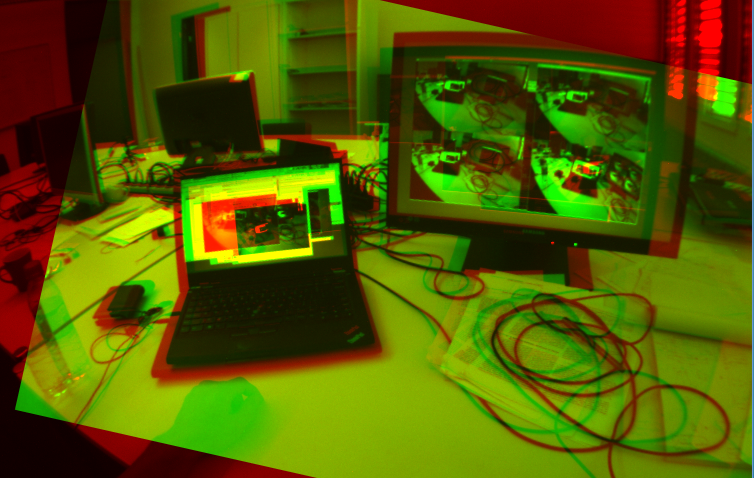
\includegraphics[width=8cm]{img/se2_error_1.png}
  \caption{$SE(2)$ transformation error visualization}
  \label{fig:se3_error_1}
\end{figure}


\subsubsection{Alternative Real Pose Finder}
\label{ssub:real_pose_finder_alternative}

During the mapping of an area, the VO algorithm finds landmarks in the world frame which are associated with detected featured points in keyframes (i.e. every featured point in an image is related to a $3D$ position in the world frame). Given a new image, some extracted featured points can be related to a keyframe using descriptor-matching which at the same time are related to world positions. From this information the full 6 DoF translation $SE(3)$ can be computed using the prospective three-point algorithm (P3P).\\

\begin{figure}[htpb]
  \centering
  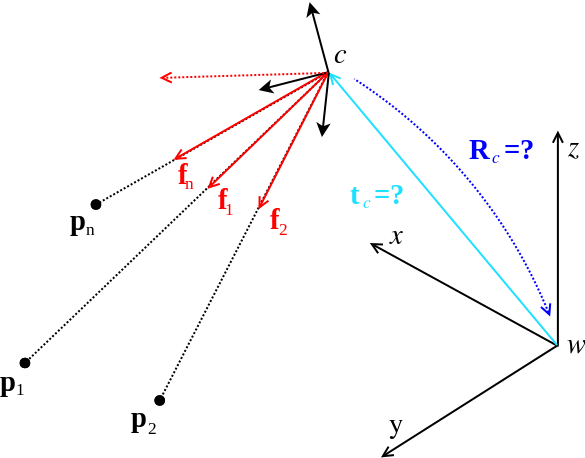
\includegraphics[width=0.6\linewidth]{img/absolute_central.png}
  \caption{From camera frame vectors $f$ (or image pixels if the camera calibration is available) and fix points $p$ the transformation between the two coordinate frames can be computed using the P3P algorithm. Image taken from \cite{kneipopengv}}
  \label{fig:img/absolute_centra}
\end{figure}

First, descriptors from every featured point are extracted. Second, a brute force KNN matching is performed from all the extracted descriptors from on image and all the descriptors of the second image. The first, and second most similar descriptor are retrieved. Then, only good matches are kept, that is, using the matching technique described by Lowe~\cite{lowe2004distinctive}, only matches with a descriptor ratio between the first and the second closest match of 0.8 or less are kept.\\

Finally, the three-point algorithm is fed with the pixel positions from the query image and the landmarks from the other. Because there are still outliers after the described simple filtering, this process is run in RANSAC~\cite{fischler1981random} framework. \\


Figures~\ref{fig:3pt_matches} is an example of the described above.\\

\begin{figure}[htpb]
  \centering
  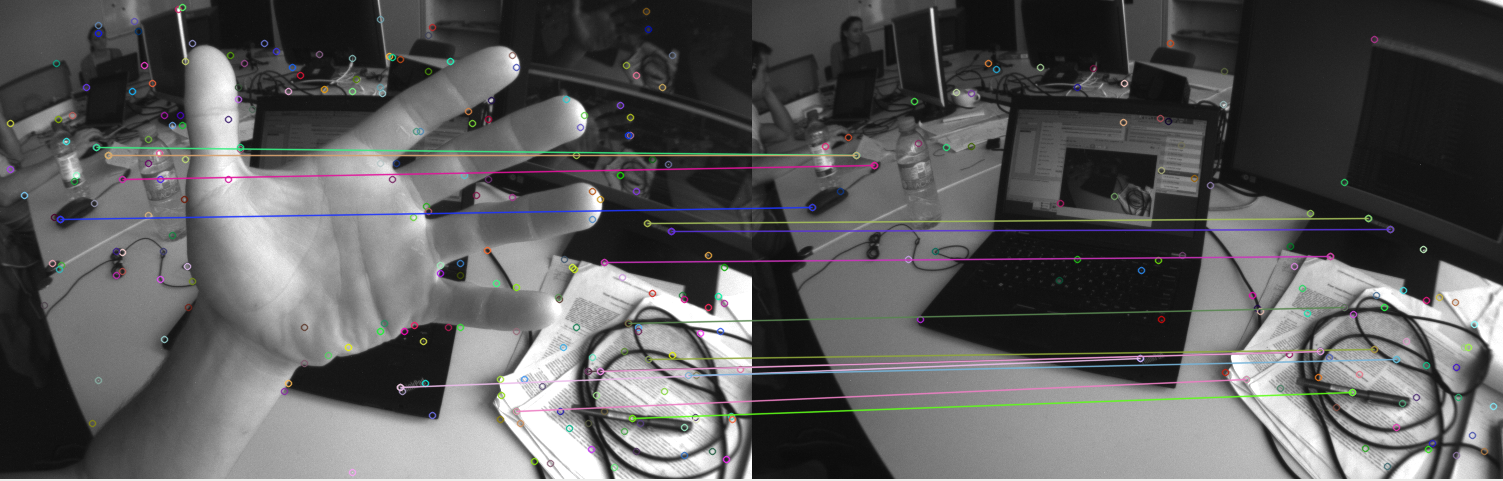
\includegraphics[width=1.0\linewidth]{img/3pt_matches_1.png}
  \caption{Accepted matches using SIFT}
  \label{fig:3pt_matches}
\end{figure}


\section{Using ferns}
\label{sec:using_ferns}

As said previously with the three-point algorithm it is possible to recover the 6 DoF of the camera pose from the relation from pixel coordinates and points in space. In this case machine learning techniques are used to model this relationship. In the classifier scheme, an object in space is a class and multiple views seen from the camera should all be classified as this class.\\

A \textit{fern}~\cite{Ozuysal2010} is a descriptor made from a set of binary tests such as in equation~\ref{eq:fern_test}. When used as a classifier, every possible evaluation of a \textit{fern} will contain a posterior probability distribution for every class.\\

\begin{equation}
  f_j =
  \left\{
    \begin{array}{l l}
      1, & \text{if} \quad I(d_j,1) < I(d_j,2) \\
      0, & \text{otherwise}
    \end{array} \right.
  \label{eq:fern_test}
\end{equation}


One \textit{fern} is usually not descriptive enough to correctly classify. In~\cite{Ozuysal2010} it is claimed that with 50 \textit{ferns} and $S=11$ a problem with 200 different classes is tractable. Regarding storage requirements, it would involve $50\times2^{11}\times200 = 20480000$ elements to be stored in memory. If these are stored as \textit{float} then 78 MB are needed, which is tractable. \\


%! TEX root = paper.tex

\section{Results}
\label{sec:results}

The descrived methods have been tested in a desktop scene covering an area of 7x3 meters. The path taken to acquire training and testing data covering the mentioned area can be seen in~\ref{fig:large_desktop_train_test}. The dataset contains 84 frames for training and 69 for testing.\\

\begin{figure}[htpb]
  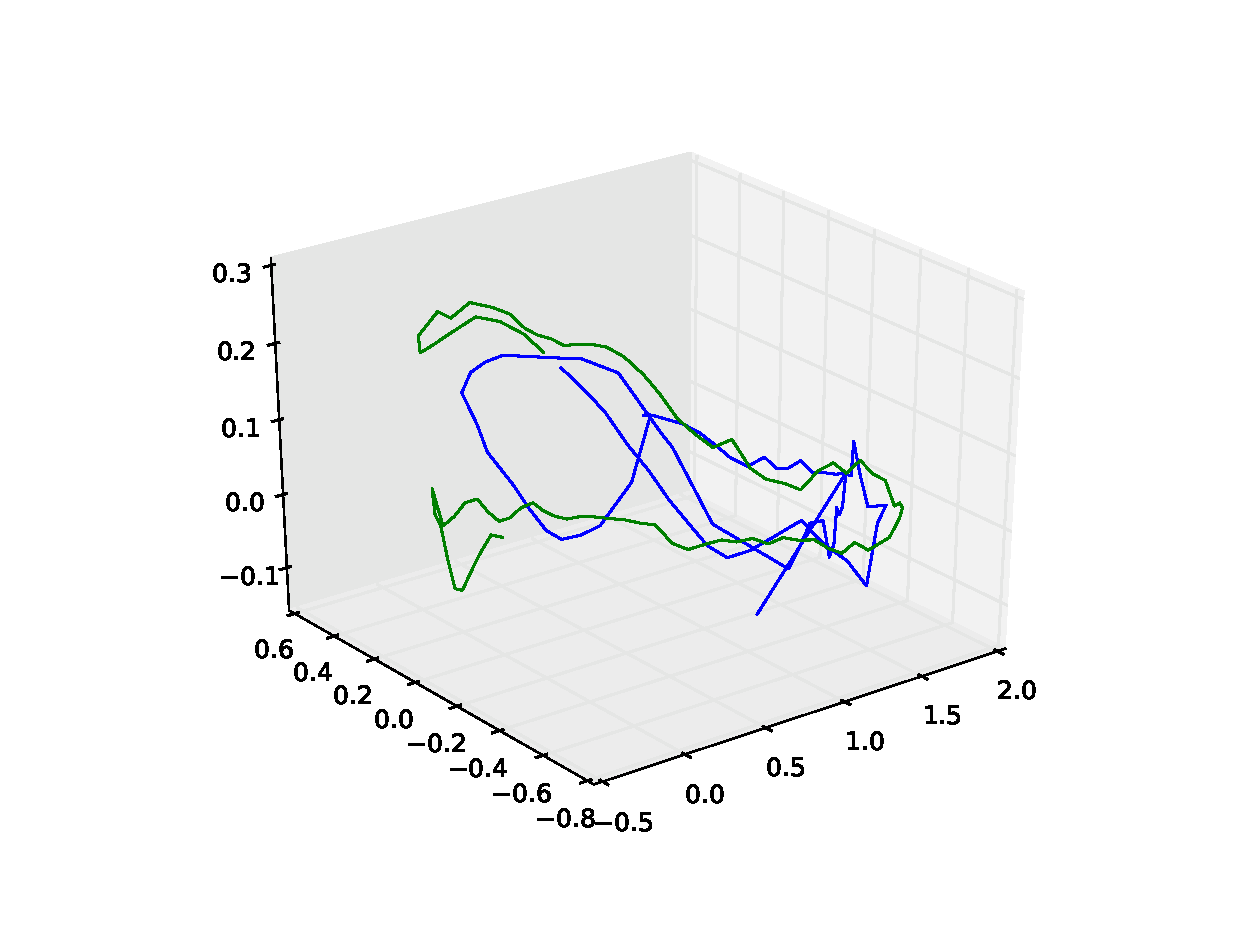
\includegraphics[width=\linewidth]{img/large_desktop/test_train_path.eps}
  \caption{In green, the path used for training. In blue, the path used for testing}
  \label{fig:large_desktop_train_test}
\end{figure}

\subsection{Multi Relocalizer}
\label{sub:multi_relocalizer_large}


\subsubsection{Extended Second-order Minimization \textit{Real Pose Finder}}
\label{ssub:extended_second_orther_minimization_real_pose_finder}

The performance of ESM Real Pose Finder is not great in this dataset as seen in~\ref{fig:desktop_2_CC_3pt_dist_1} although it was able to correctly relocalize in other datasets.\\

\begin{figure}[htpb]
  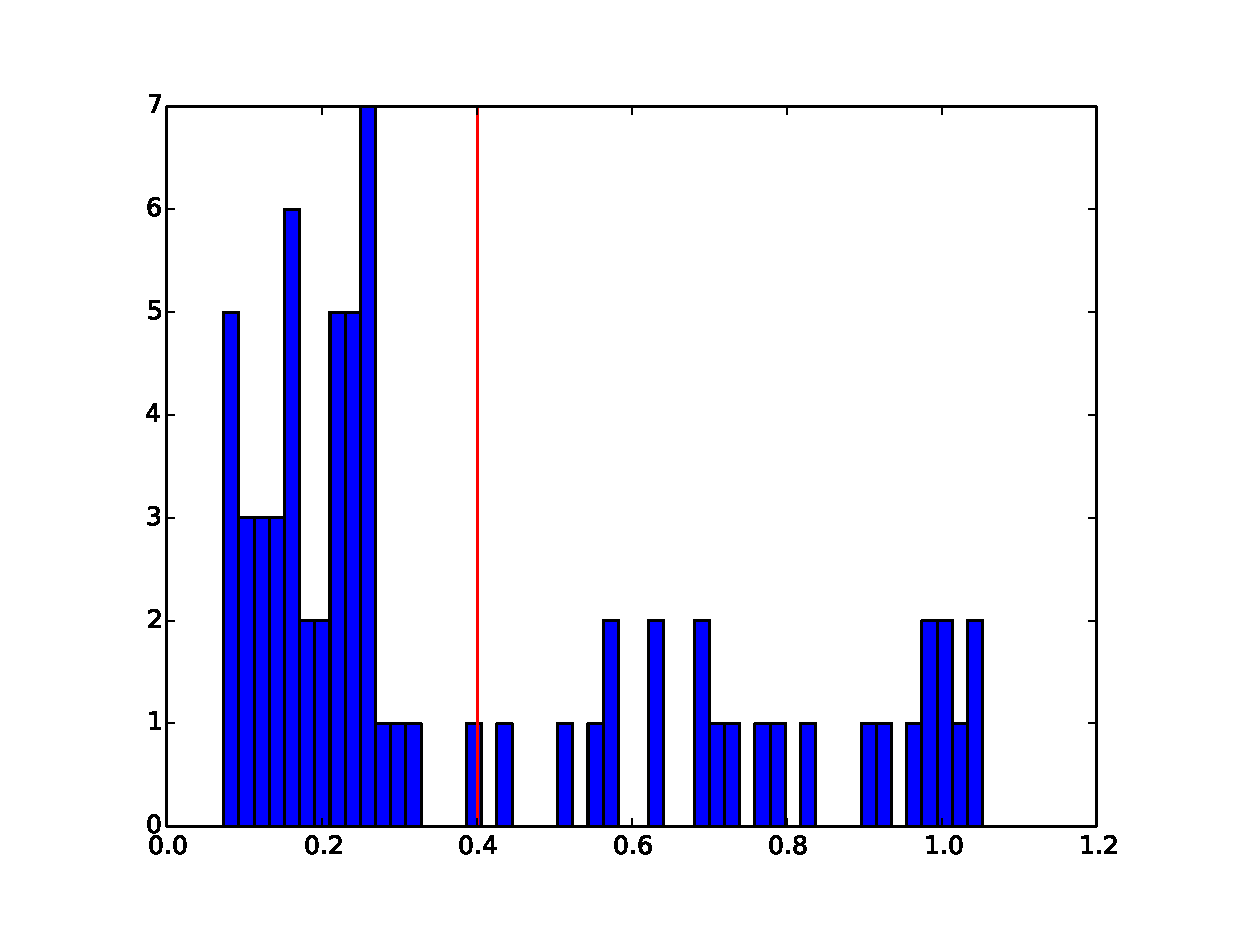
\includegraphics[width=1\linewidth]{img/large_desktop/CC_esm_dist.eps}
  \caption{Translation error histogram using CC \textit{Place Finder} and ESM \textit{Real Pose Finder}}
  \label{fig:desktop_2_CC_esm_dist_1}
\end{figure}


\subsubsection{Three-point \textit{Real Pose Finder}}
\label{ssub:large_three_point_real_pose_finder}

On the other side, the Three-point \textit{Real Pose Finder} works very well as seen in~\ref{fig:desktop_2_CC_3pt_dist_1}. It can correctly retrieving the pose of 42 of the 69 frames. This method is very dependent on the results of the \textit{Place Finder}, and on this dataset, the cross correlation method was not very effective. Better results on it would help iprove the results of this method and the ESM method.\\

\begin{figure}[htpb]
          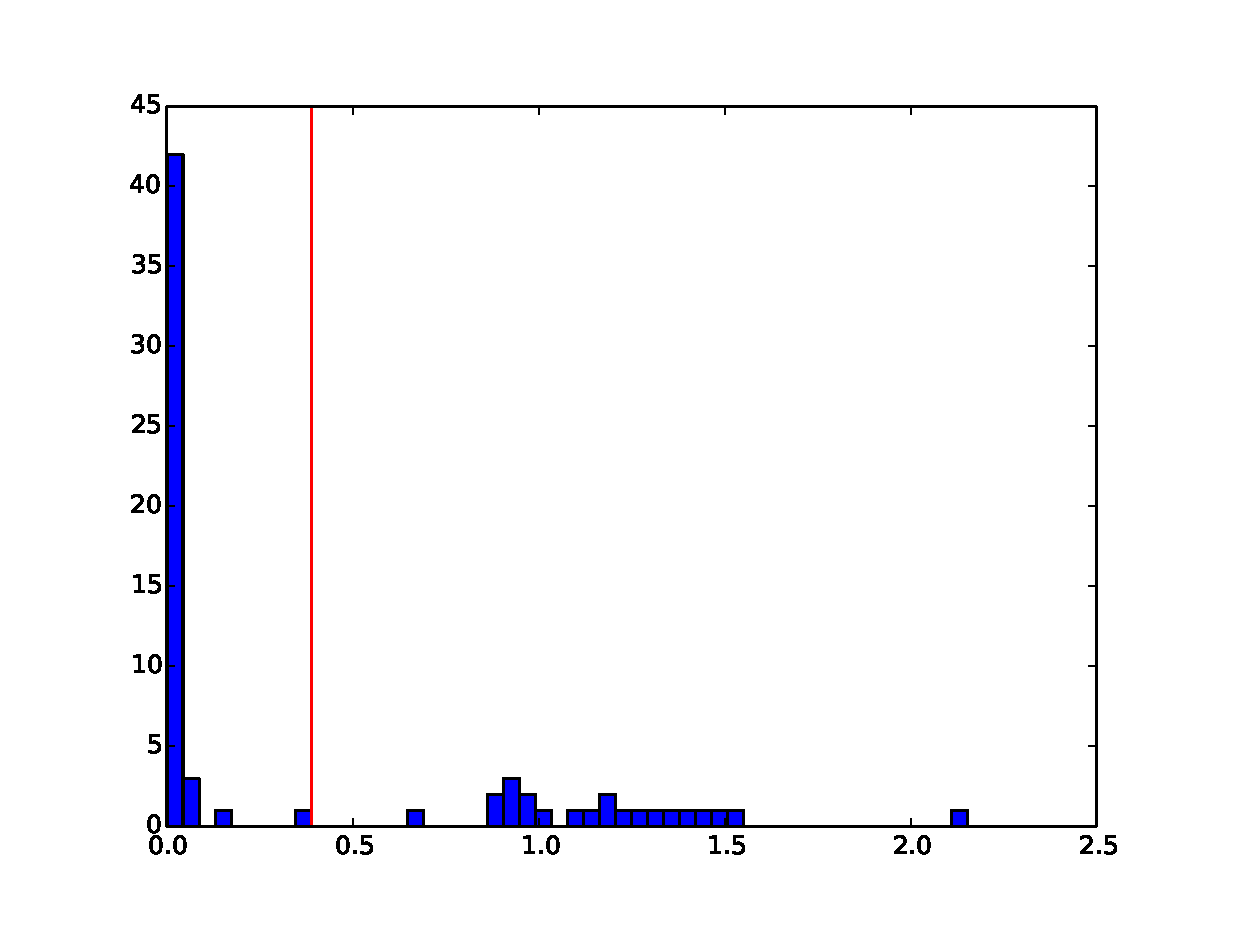
\includegraphics[width=1\linewidth]{img/large_desktop/CC_3pt_dist.eps}
          \caption{Translation error histogram using CC and P3P, with the mean marked as a red line}                
          \label{fig:desktop_2_CC_3pt_dist_1}
\end{figure}


\subsection{Ferns}
\label{sub:large_ferns}

Finally, as an alternative to the PTAM relocalization method, it was proposed to use machine learning techniques, more concretely \textit{ferns}. In~\cite{Ozuysal2010} it is shown that \textit{ferns} can be used to distinguish up to around 200 different classes. We applied the method to this dataset where there are 1730 classes. In figure~\ref{fig:large_desktop_ferns_dist} it can be seen that almost 50 of the 69 frames where correctly relocalized. Which is more than using Multi Relocalizer with the three-point \textit{Real Pose Finder}. The classifier was trained with 100 \textit{ferns} of 12 tests each.\\

It should be noticed that not all points need to be well classified, as long as more than 3 points are correctly identified then the posterior RANSAC will find and use the once that agree.\\

The three-point with CC method and this one, can correctly relocalize the same number of frames. Probably there is one part of the dataset that is more ambiguous and difficult to recognize and both algorithms struggle with it.\\

\begin{figure}[htpb]
          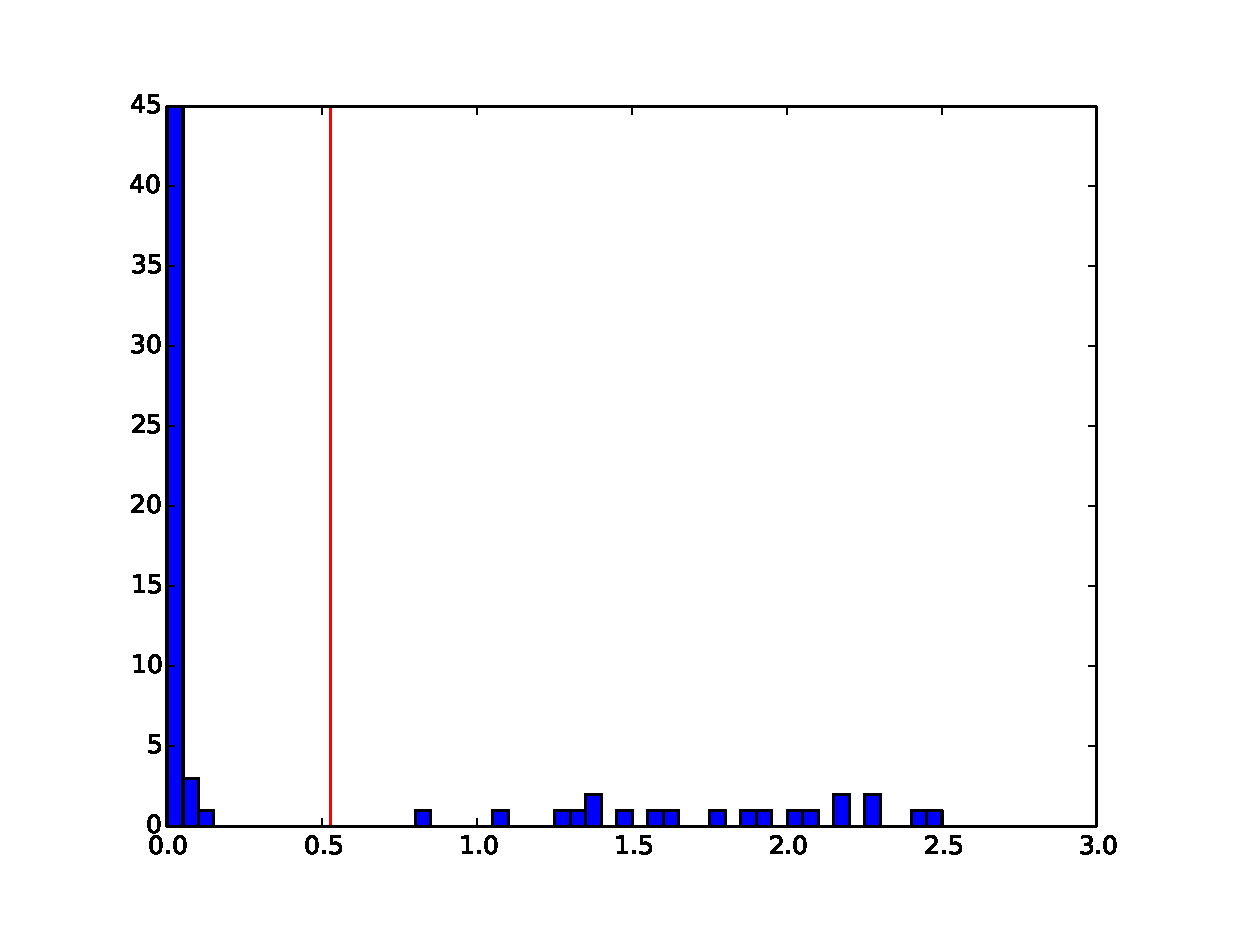
\includegraphics[width=1\linewidth]{img/large_desktop/ferns_100_dist.eps}
          \caption{Translation error histogram using \textit{ferns} with 12 tests, with the mean marked as a red line}                
          \label{fig:large_desktop_ferns_dist}
\end{figure}

\section{Execution time}
\label{sec:execution_time}

In figure~\ref{fig:exec_time} the mean execution time of relocalization is shown. There, it can be seen that the ESM and the P3P methods are the faster while the method using \textit{ferns} classifier is slower and is sensitive to the number of classes. Also, while ESM and P3P use optimized third party libraries, the \textit{ferns} based classifier has been integrally implemented by us, maybe not achieving the best performance. The used training time for the classifier can be seen in figure~\ref{fig:training_time}.\\

\begin{figure}[htpb]
  \centering
  \begin{bchart}[steps={0.2,0.4,0.6,0.8,1},max=1, scale=0.6]
  \bcbar[label= CC and ESM]{0.0437}
  \bcbar[label=CC and P3P]{0.0647}
  \bcbar[label=ferns 237 classes]{0.128}
  \bcbar[label=ferns 1730 classes]{0.933}
  \end{bchart}
  \caption{Single relocalization execution time}
  \label{fig:exec_time}
\end{figure}


\begin{figure}[htpb]
  \centering
  \begin{bchart}[step=10, max=70, scale=0.6]
    \bcbar[label=\quad 237 classes]{5.57}
    \bcbar[label=1730 classes]{63.11}
  \end{bchart}
  \caption{\textit{ferns} classifier training time}
  \label{fig:training_time}
\end{figure}

%! TEX root = thesis_pres.tex

\section{Discussion}
\subsection{Conclusions}
\label{sub:conclusions}

\begin{frame}[t]{Conclusions}
  \begin{block}{Work done}

    \begin{itemize}
      \item We have addressed one of the missing parts of SVO
      \item Different methods have been studied an evaluated
      \item An independent framework and library have been implemented
    \end{itemize}

  \end{block}
  \begin{block}{Future work}
    \begin{itemize}
      \item Further tests on board
      \item Use image retrieval techniques like bag of word as Place Finder
      %\item Further investigation and improvements on Machine Learning techniques 
      \item Test performance on rectified images
    \end{itemize}

  \end{block}

\end{frame}

\begin{frame}[t]{Thank you!}
  \vfill
  \centering{Questions?}
  \vfill

\end{frame}


\begin{frame}[t]{Bibliography}
  \bibliographystyle{abbrv}
  \bibliography{../rpg_templates/thesis_template/bibtex/references}
\end{frame}

\end{document}
